\chapter{Word Embeddings}
\section{Introduction}
A very basic definition of a word embedding is a real number, vector representation of a word. Typically, these days, words with similar meaning will have vector representations that are close together in the embedding space (though this hasn\rq t always been the case).

\begin{figure}[H]
    \centering
    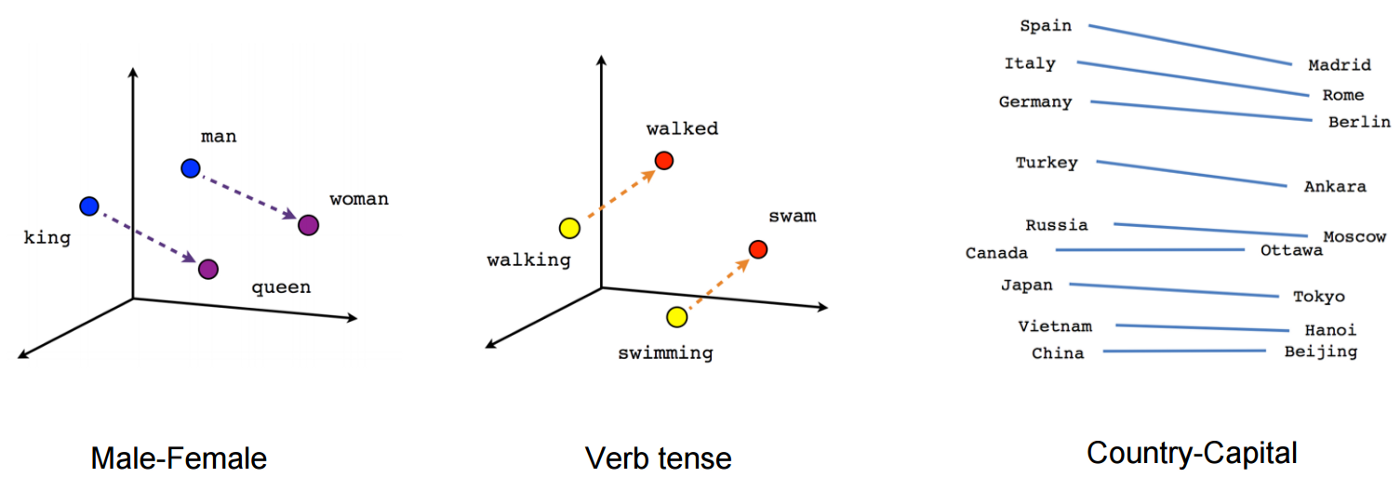
\includegraphics[scale = 0.33]{word2vec.png}
    \caption{Word2Vec}
    \label{fig:word2vec}
\end{figure}

When constructing a word embedding space, typically the goal is to capture some sort of relationship in that space, be it meaning, morphology, context, or some other kind of relationship.

By encoding word embeddings in a densely populated space, we can represent words numerically in a way that captures them in vectors that have tens or hundreds of dimensions instead of millions (like one-hot encoded vectors).

Different word embeddings are created either in different ways or using different text corpora to map this distributional relationship, so the end result are word embeddings that help us on different down-stream tasks in the world of NLP.

\section{Why Word Embeddings? }
Words aren\rq t things that computers naturally understand. By encoding them in a numeric form, we can apply mathematical rules and do matrix operations to them. This makes them amazing in the world of machine learning, especially.

Take deep learning for example. By encoding words in a numerical form, we can take many deep learning architectures and apply them to words. Convolutional neural networks have been applied to NLP tasks using word embeddings and have set the state-of-the-art performance for many tasks.

Moreover, word embeddings can be pre-trained and can be used for variety of NLP applications like text classification, question-answering, auto-complete, spelling correction, speech processing, etc.

\section{Word Embeddings Methods}
\subsection{One-Hot Encoding(Count Vectorizing)}
One of the most basic ways we can numerically represent words is through the one-hot encoding method (also sometimes called count vectorizing).

In one-hot encoding, to represent a word, a vector of dimension equal to the number of unique words in the corpus is created. Each unique word has a unique dimension and will be represented by 1 in that dimension with 0s everywhere else.

Let, \textbf{Corpus : } \{I have a pen\}

Then, the vector representation of words will be

\textbf{I : } [1, 0, 0, 0]

\textbf{have : } [0, 1, 0, 0]

\textbf{a : } [0, 0, 1, 0]

\textbf{pen : } [0, 0, 0, 1]

As in above example, each unique word is assigned a vector with its dimension equal 1 and all other equal 0.

Disadvantage of one-hot encoding is words are represented by huge and sparse vectors that captures no relational information.

\subsection{Word2Vec}
In 2013, with Word2Vec , Mikolov et al. at Google completely changed the embedding paradigm: from then on, embedding will be the weights of a neural network that are adjusted to minimize some loss, depending on the task. Embedding had become a neural network algorithm.

Word2vec is not a singular algorithm, rather, it is a family of model architectures and optimizations that can be used to learn word embeddings from large datasets. Embeddings learned through word2vec have proven to be successful on a variety of downstream natural language processing tasks.

There are two major learning approaches for Word2Vec.

\subsubsection{Continuous Bag-of-Words (CBOW)}
It predicts the middle word based on surrounding context words. The context consists of a few words before and after the current (middle) word. This architecture is called a bag-of-words model as the order of words in the context is not important.

\begin{figure}[h]
    \centering
    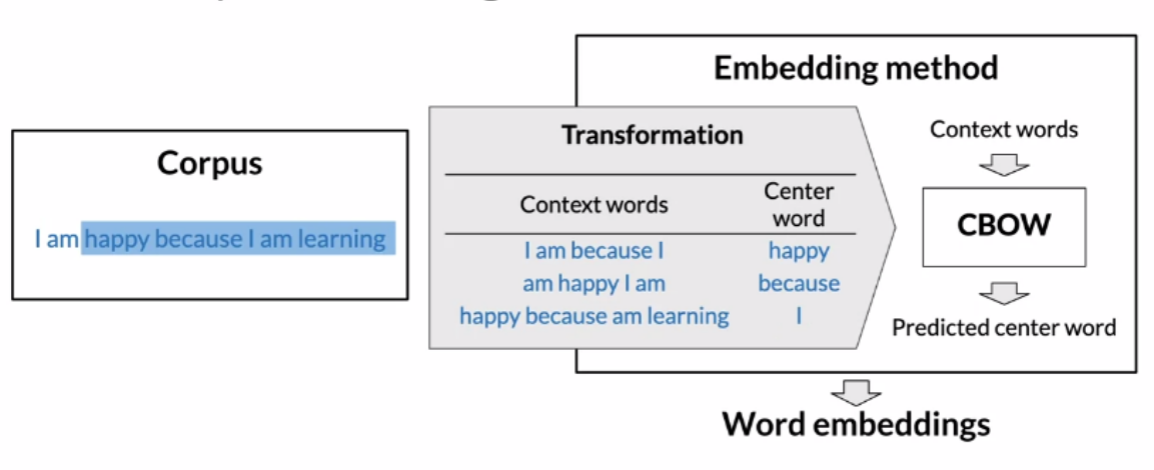
\includegraphics[scale = 0.33]{CBOW.png}
    \caption{CBOW Model}
    \label{fig:CBOW}
\end{figure}


\subsubsection{Continuous Skip-Gram}
This method learns an embedding by predicting the surrounding words given the context. The context is the current word.

Both of these learning methods use local word usage context (with a defined window of neighboring words). The larger the window is, the more topical similarities that are learned by the embedding. Forcing a smaller window results in more semantic, syntactic, and functional similarities to be learned.

Using Word2Vec model, high quality embeddings can be learned pretty efficiently, especially when comparing against neural probabilistic models. That means low space and low time complexity to generate a rich representation.

More than that, the larger the dimensionality, the more features we can have in our representation. But still, we can keep the dimensionality a lot lower than some other methods. It also allows us to efficiently generate something like a billion word corpora, but encompass a bunch of generalities and keep the dimensionality small.


\subsection{GloVe}
GloVe is an extension of word2vec, and a much better one at that. There are a set of classical vector models used for natural language processing that are good at capturing global statistics of a corpus, like LSA (matrix factorization). They\rq re very good at global information, but they don\rq t capture meanings so well and definitely don\rq t have the cool analogy features built in.

\begin{figure}[H]
    \centering
    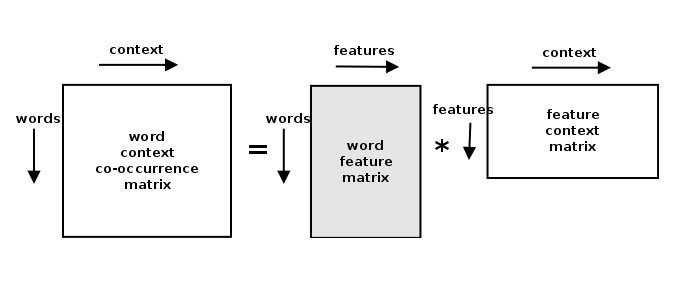
\includegraphics[scale = 0.7]{Glove.png}
    \caption{Glove Model}
    \label{fig:Glove}
\end{figure}

GloVe\rq s contribution was the addition of global statistics in the language modeling task to generate the embedding. There is no window feature for local context. Instead, there is a word-context/word co-occurrence matrix that learns statistics across the entire corpora.


\subsection{Others}
Some other word embedding methods are fastText(Facebook, 2016), BERT (Google, 2018), ELMo(Allen Institute for AI, 2018) and GPT-2(OpenAI, 2018).

\section{Feature Vectors and Similarity Scores}

Word vectors represent words in a way that encodes their meaning. A vector is simply an array of fractions. Here\rq s a vector taken from the Google News model. It\rq s the vector for the word “fast”. It consists of 300 floating point values: [0.0575, -0.0049, 0.0474, ......, -0.0439]

The straight line distance between two points is called the “Euclidean” or “L2” distance, and it can be extended to any number of dimensions. Here\rq s the formula for the distance between two vectors a and b with an arbitrary number of dimensions (n dimensions):

\begin{equation}
    dist_{L2}(a, b) = \sqrt{\sum_{i = 0}^{n} (a_i - b_i)^2}
\end{equation}


Here\rq s the important insight, word2vec learns a vector for each word in a vocabulary such that words with similar meanings are close together and words with different meanings are farther apart. That is, the Euclidean distance between a pair of word vectors becomes a measure of how dissimilar they are.

The Euclidean distance is what we intuitively understand as distance, and it\rq s a workable distance metric for comparing word vectors, but in practice another metric called the Cosine similarity gives better results.

\begin{equation}
    Similarity(A, B) = \frac{A.B}{|| A || * || B ||} = \frac{\sum_{i = 1}^{n} A_i * B_i}{\sum_{i = 1}^n A_i^2 * \sum_{i = 1}^n B_i^2}
\end{equation}

The Cosine similarity between two vectors a and b is found by calculating their dot product, and dividing this by their magnitudes. The cosine similarity is always a value between -1.0 and 1.0.

\section{Data Cleaning and Tokenization}
Following details should be followed for proper word embedding while data pre-processing and tokenization.

\begin{enumerate}
    \item \textbf{Letter case :}
          In enligsh language, the letter case (eg: \lq Eagle\rq or \lq eagle\rq) doesn't change the meaning of the words. Hence, it is better to have all data in lower case for word embedding.

    \item \textbf{Punctuation :}
          Punctuation symbols like ", ', !, ?, etc. should be handled before word embeddings.

    \item \textbf{Numbers :}
          Numbers (0, 1, 2, 3 ....) should be removed before word embeddings if they are not important for semantic meaning.

    \item \textbf{Special characters :}
          Special characters like $\delta , \Delta , \alpha , \beta , $ etc. should be handled before word embeddings.

    \item \textbf{Special words :}
          Special words like \lq\#nlp\rq, emojis, etc. should be cleaned.
\end{enumerate}

\section{Evaluation of Word Embeddings Model}
\subsection{Extrinsic Evaluation}
In extrinsic evaluation, word embeddings are tested on external tasks like named entity recognition, parts-of-speech tagging, etc. It evaluates the actual usefulness of embeddings. However, it is time consuming and more difficult to troubleshoot.

\subsection{Intrinsic Evaluation}
Similarity and analogy test are used for intrinsic evaluation. 




